\chapter{Introduction} \label{chap:intro}
This work is focused on the studies, measurements and corrections of linear optics and betatron coupling applied during Sirius storage ring commissioning. Sirius is the new Brazilian 4\ts{th} generation synchrotron light source. 

The content of this dissertation is the following:
\begin{itemize}
    \item Chapter 1: an introduction to the general concepts related to synchrotron light sources, the Sirius Project, the scientific background and main objectives.
    \item Chapter 2: the basic accelerator physics theory that is necessary for the development of the work.
    \item Chapter 3: the theory related to the Linear Optics from Closed Orbits (LOCO) method and the code implementation for Sirius.
    % \item Chapter 4: a discussion on LOCO method implementation in Python for the Sirius storage ring and the tests performed with simulated data.
    \item Chapter 4: the application of LOCO method with data obtained in Sirius storage ring during commissioning, presenting and discussing the linear optics and coupling measurements and its corrections.
\end{itemize}

In this chapter, general concepts and the terminology regarding synchrotron light sources will be introduced in Section~\ref{sec:sls}. The main information about the Sirius project will be presented in Section~\ref{sec:sirius_project}. The scientific background related to the studies conducted in this work is discussed in Section~\ref{sec:background} and the goals are exhibited in the final Section~\ref{sec:master_obj}.
\section{Synchrotron Light Sources}\label{sec:sls}
Charged particles at relativistic speeds radiate synchrotron light when accelerated perpendicularly to its direction of motion~\cite{jackson}. Synchrotron light sources are scientific facilities where this effect is ultimately exploited in order to produce light with high brightness and covering a broad energy range, with a spectrum from infrared light up to hard X-rays. The synchrotron light sources are high quality and versatile scientific tools that allow for a great diversity of high resolution experiments in several research areas, such as materials sciences, condensed matter physics, nanotechnology and many others.

Generally a synchrotron light source is composed by three main systems\footnote{Throughout this dissertation the set of the accelerator systems in the synchrotron also may be referred as the ``machine''.}: the injection system, the storage ring and the beamlines. Typically the charged particles used in these facilities are electrons. A brief description of each subsystem can be made:
\begin{description}[align=left]
    \item[Injection system:] composed by an electron source, a~\gls{linac}, a synchrotron, generally called booster, and transport lines connecting the accelerators. The electrons are emitted from an electron gun and accelerated by~\gls{rf} structures along the~\gls{linac}. Then the electrons are injected in the first circular accelerator, the booster, where their energy is ramped up to the storage ring's energy\footnote{In some facilities, the beam is injected from the~\gls{linac} directly to the storage ring, where the energy ramp is performed.}.
    \item[Storage ring:] after beam extraction from the booster ring, the ultra-relativistic electrons are injected in the second circular accelerator, the storage ring, where electromagnetic fields are used to confine the electrons in stable closed orbits for many hours inside a vacuum chamber with ultra-high vacuum. In this approximated circular orbits the electrons produce synchrotron light that is supplied to the beamlines.
    \item[Beamlines:] experimental stations installed tangentially to the storage ring, where the generated synchrotron light is used in a wide variety of scientific studies based on the radiation-matter interactions.
\end{description}

Typical values for the ``low'' energy obtained in the~\gls{linac} are hundreds of \si{\mega\electronvolt} and the ``high'' nominal energy in the storage ring are usually few \si{\giga\electronvolt}. The whole injection process occurs with a repetition rate of a few \si{\hertz} until the storage ring is filled with electrons, reaching the operation current. The injection events might occur only in specific times of the day and in this case the storage ring operates in the so-called decay mode. The injection system may also fill the storage ring more frequently to keep the stored current almost constant during operation, this is called top-up mode.

The quality of the radiation produced in synchrotron light sources can be measured by the quantity called brightness. It is a measure of the radiation intensity, source size and collimation for a given energy and can be defined as~\cite{huang2013}:
\begin{equation}
    B(\omega) = \dfrac{F(\omega)}{\Sigma_x \Sigma_{x'} \Sigma_y \Sigma_{y'} \left(\Delta \omega /\omega\right)}.
\end{equation}

The photon frequency $\omega$ and the photon energy are related by $E = \hbar \omega$. The photon flux is represented by $F(\omega)$ and it is the number of photons per second. The products $\Sigma_x \Sigma_{x'}$ and $\Sigma_y\Sigma_{y'}$ are the photon beam volumes in the horizontal and vertical phase space, respectively. The frequency bandwidth $\Delta \omega/\omega$ considered in the brightness calculation is typically $0.1\%$. The photon beam volume in phase space depends both on the photon and the electron distributions. The electron beam volume in phase space is called beam emittance and it is a property derived from the storage ring magnetic lattice.

In order to achieve high brightness for a synchrotron light source, one must increase the photon flux by increasing the electron current and also minimizing the electron beam emittance. Constant advances both in the theoretical and technological aspects have been made in the accelerator community in the last decades, allowing for tremendous gains in brightness of synchrotron light sources\cite{eriksson, liu2017}. 

Such great increments in brightness scales have made it possible to classify the synchrotron light sources in generations. The 1\ts{st} synchrotron light source generation appeared in the early 1960's as a parasitic effect from the bending magnets in particle colliders. The 2\ts{nd} generation in the 1980's were dedicated light sources built for the production of synchrotron radiation, generated mainly by bending magnets. The 3\ts{th} generation light sources in the 1990's were optimized to produce synchrotron radiation with \glspl{id} installed in long straight sections in the storage ring~\cite{liu2017}. The \glspl{id} are arrays of magnetic blocks organized in an alternated manner such that the electron beam follows a transversely undulating path when it passes through the device. The sequence of transverse accelerations induce the electrons to radiate synchrotron light, which may interfere to produce a photon beam with very high intensity and a sharp spectrum, as compared to the light emitted at the dipoles. Depending on the magnetic fields in the~\gls{id}, the polarization of the emitted radiation can also be varied. The \glspl{id} types commonly used in 3\ts{th} synchrotrons are wigglers and undulators.

In~\glspl{4gsr}, recent developments in the accelerator field have been applied to reduce the electron beam emittance by orders of magnitude as compared to the previous generation, thus increasing the brightness accordingly. Modern undulators are also used as \glspl{id} in the storage ring long straight sections. The beginning of the 4\ts{th} generation of synchrotron storage rings was marked by the commissioning of MAX-IV in 2015~\cite{eriksson2016}, the first~\gls{4gsr} implemented. A brief overview about the main ideas applied in~\glspl{4gsr} will be given in Subsection~\ref{subsec:fourth_generation}.
% Presently, these modern storage rings deliver synchrotron light to the beamlines with the highest brightness and coherence flux ever achieved in the history of synchrotron light sources. 
\subsection{Main Devices in a Storage Ring}\label{subsec:devices}
Magnetic fields are used to deflect and focus the electron beam in the storage ring. Each type of magnetic field is used for a certain purpose and is created by different types of magnets installed around the ring, which form the so-called magnetic lattice. Typically the magnetic lattice is composed by electromagnets with coils fed by power supplies but it is also possible to use permanent magnets. The main magnets types and their functions are:
\begin{description}
    \item[Dipoles:] bending magnets that create an approximated constant magnetic fields which are used to radially deflect the electrons in curved paths, totalling a $\SI{2\pi}{\radian}$ deflection in one turn and allowing for a closed orbit motion.
    \item[Quadrupoles:] focusing magnets that provide magnetic fields whose intensity is linearly dependent on the electron transverse deviations. These magnetic fields create a deflection with a strength determined by the deviation from the reference orbit. From the Lorentz force expression it can be obtained that if a quadrupolar field is focusing in one direction it is necessarily defocusing in the perpendicular direction. Thus, to obtain a net focusing in both directions, an alternated focusing scheme must be used with two types of quadrupoles: focusing and defocusing. The electron dynamics in the presence of dipolar and quadrupolar fields is linear, then the magnetic lattice constituted only by dipoles and quadrupoles is also denominated as a linear lattice.
    \item[Sextupoles:] electrons with energy deviations from the storage ring nominal energy are differently focused in a linear magnetic lattice. Since the electrons in a beam have an energy distribution, chromatic aberrations effects may disturb the electrons stability. The sextupoles create magnetic fields that depend quadratically on the electron tranverse deviations, therefore it introduces focusing forces that depends on the transverse displacements and allows for the correction of these chromatic aberrations. However, the non-linear fields introduced by the sextupoles also change the beam dynamics to a non-linear regime and the motion of electrons with sufficiently large deviations may be unstable. The largest deviations that still produce a stable motion define a region in the electron phase space called dynamic aperture. Hence, more sextupoles must be included in the lattice in order to increase the stability region, i.e., increase the storage ring dynamic aperture. For the same reason as for the quadrupoles, two types of sextupoles, focusing and defocusing, are needed to correct the chromatic effects in both transverse planes.
\end{description}

Figure~\ref{fig:magnets} shows a schematic representation of the magnet blocks and the corresponding field lines for each type of magnet. In these examples, the electron path points inwards the paper (or screen), the radial positive direction is pointing to the left and the vertical positive direction to the upper side. In this way, the exemplified quadrupoles and sextupoles are defined as focusing (it focus the beam in the radial direction) and the corresponding defocusing types are obtained by a $\SI{\pi/2}{\radian}$ rotation for quadrupoles and $\SI{\pi/3}{\radian}$ for sextupoles.

\begin{figure}
\centering
\begin{subfigure}[t]{0.32\textwidth}
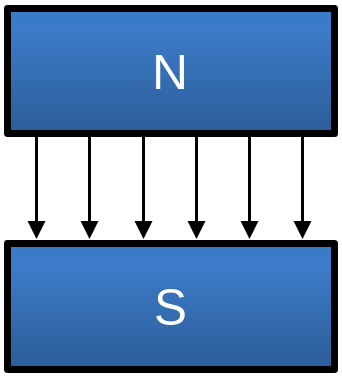
\includegraphics[width=0.9\textwidth]{figures/dipole_example.png}
    \caption{Dipole}
    \label{subfig:dipole}
\end{subfigure}
 \begin{subfigure}[t]{0.32\textwidth}
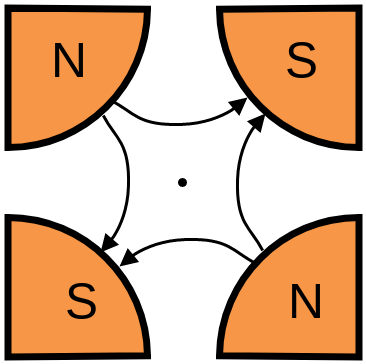
\includegraphics[width=1.0\textwidth]{figures/quadrupole_example.png}
    \caption{Quadrupole}
    \label{subfig:quadrupole}
\end{subfigure}
 \begin{subfigure}[t]{0.32\textwidth}
    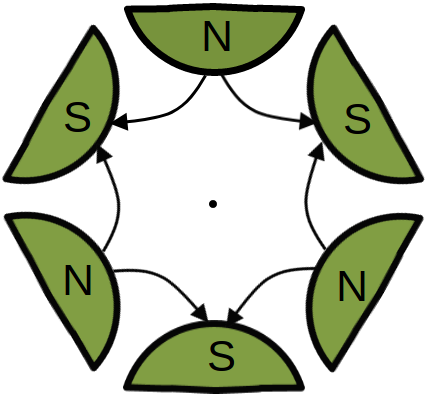
\includegraphics[width=1.08\textwidth]{figures/sextupole_example.png}
    \caption{Sextupole}
    \label{subfig:sextupole}
\end{subfigure}
\caption{Schematic examples of magnets used in storage rings.}
\label{fig:magnets}
\end{figure}

The electron beam centroid positions can be measured by devices called \glspl{bpm}, installed in the vacuum chamber at many locations around the storage ring. The measurements can be performed in a turn-by-turn basis to access the beam trajectories and also averaging the data over many turns to obtain the information about the beam orbit. A simple scheme for a typical~\gls{bpm} device is shown in Figure~\ref{fig:bpm_scheme}, where the electron path points outwards the paper.
% \begin{figure}
%     \centering
%     \begin{tikzpicture}[pin distance=7mm, pin edge=ultra thick]
%     \draw[->] (-3,0) -- (3,0)
%     node[below left] {$x$};
%     \draw[->] (0,-3) -- (0,3)
%     node[left] {$y$};
%     \draw[ultra thick] (0,0) 
%     node[circle,
%          pin=above right:$a$,
%          pin=above left:$b$,
%          pin=below left:$c$,
%          pin=below right:$d$,
%          minimum size=3.5cm]{} circle (2.0cm);
%     \end{tikzpicture}
%     \caption{BPM scheme. The $a, b, c, d$ lines represent the device antennas.}
%     \label{fig:bpm_scheme}
% \end{figure}
\begin{figure}
    \centering
    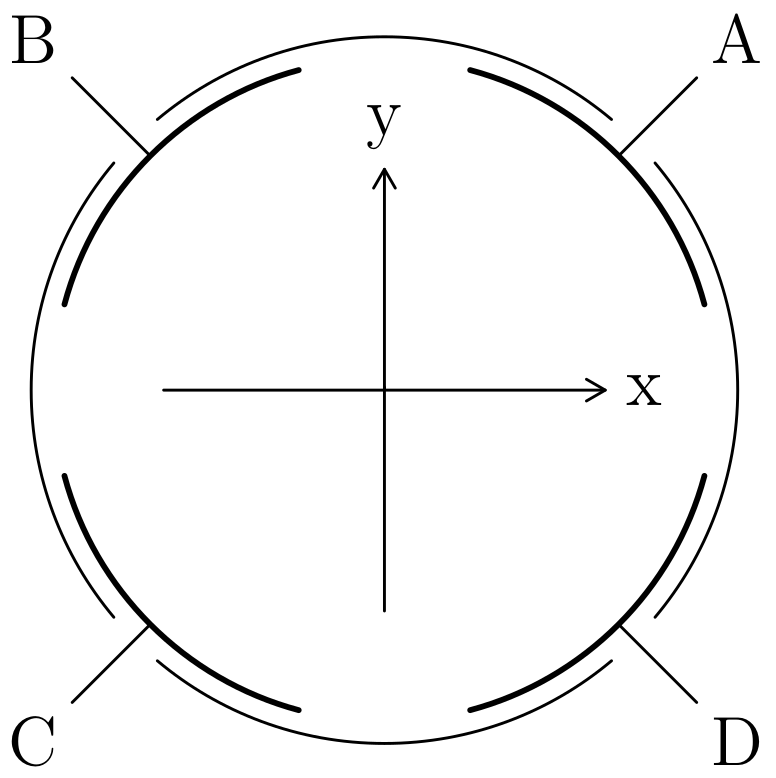
\includegraphics[width=0.35\textwidth]{figures/bpm_scheme.png}
    \caption{BPM scheme. The A, B, C, D lines represent the device antennas. Adapted from~\cite{huang2019beam}.}
    \label{fig:bpm_scheme}
\end{figure}

The electron beam excites electromagnetic signals in the four~\gls{bpm} antennas. The values of these four intensities measured at the antennas can be manipulated to calculate the transverse positions for the beam centroid:
\begin{align}
    x &= K_x \dfrac{\left(A + D\right) - \left(B + C\right)}{\Sigma_{\mathrm{BPM}}} \\
    y &= K_y \dfrac{\left(A + B\right) - \left(C + D\right)}{\Sigma_{\mathrm{BPM}}},
\end{align}
where $\Sigma_{\mathrm{BPM}} = A + B + C + D$ is the sum signal from all~\gls{bpm} antennas and it is directly proportional to the electron beam current. $K_x$ and $K_y$ are calibration factors dependent of~\gls{bpm} geometry and the distances between antennas. This method of calculation is called $\Delta/\Sigma$ and other methods are available~\cite{wikibpm}.

The orbit distortions can be corrected by applying localized dipolar fields, called dipolar kicks, to steer the beam at each turn and then steer the orbit towards a target. Short dipoles, called orbit correctors or simply correctors, are added in the lattice to produce the kicks that steer the orbit. There are two types of corretors: horizontal and vertical. The horizontal correctors create vertical dipolar fields to deflect the beam in the horizontal plane and the vertical correctors produce a horizontal dipolar fields to vertically deflect the beam.

The orbit correction can be performed by measuring the orbit distortions with the \glspl{bpm} and, based on these measurements, one can calculate and apply in the correctors the corresponding kicks variations that produce an orbit change that minimizes the measured distortion, thus steering the electron beam towards a target orbit.

Since the electrons lose energy by synchrotron radiation emission in every turn around the storage ring, an energy gain process must occur to maintain the electrons in stable motion. Ressonant cavities are used in storage rings to confine oscillating electromagnetic fields with a frequency in the~\gls{rf} range. These devices are called~\gls{rf} cavities and they provide the energy gain to the electrons with longitudinal electric fields. There is a fundamental principle, called phase stability, that ensures the synchronization between the fields oscillation inside the cavity and the circulating periodic motion of the electrons. This fundamental mechanism, that is further discussed on Chapter 2, is the origin for the name ``synchrotron''.
\subsection{4\ts{th} Generation Storage Rings}\label{subsec:fourth_generation}
A magnetic lattice is composed by a sequence of magnets, called unit cells, that are repeated around the storage ring. The unit cells are connected by straight sections, without magnets. These straight sections are used for the installation of \glspl{id}. At the ends of each unit cell there are quadrupoles for the optics functions matching in the straight sections.

A new generation of synchrotron light sources emerged from the realization of innovative magnetic lattices where very small emittances can be achieved. These magnetic lattices are named~\gls{mba}, where dipoles are interspersed with quadrupoles and sextupoles, forming the arc sections, without much drift spaces between magnets. In the previous generation, the number of dipoles in a unit cell was less than four, being usually Double or Triple-Bend-Achromat lattices. For~\gls{mba} lattices there are more than four dipoles per unit cell, which explains the term ``Multi-Bend''. Since the dipoles can be viewed as spectrometers as well, they introduce a dependence of electron position with its energy. The focusing strengths in a MBA lattice are adjusted to locally correct this dispersion effects, allowing for independence on position with energy in the straight sections and this is what the term ``Achromat'' refers to. 

The natural emittance of a storage ring depends on the electron energy and the number of dipoles in the lattice roughly as $\epsilon \propto \gamma^2/N_{b}^3$. For a fixed circumference, more dipoles in a magnetic lattice implies that the individual bending angles may be reduced, therefore reducing the energy dispersion errors created by these magnets. The equilibrium emittance depends on the dispersion effects at dipoles, so minimizing the dependence on electron position with energy at the bending magnets is one of the key factors to reduce the natural emittance.

The seemingly simple idea related to the MBA magnetic lattice was proposed in the early 1990's~\cite{einfeld1993} but it took more than 20 years to be implemented in practice due to the related accelerator technology and engineering challenges that needed to be overcome~\cite{hettel}. The technical problems appear in a cascade-effect fashion. Quadrupoles with strong focusing strengths are required in order to locally correct the energy dispersion errors created by several dipoles in a compact arc section. With strong focusing strengths comes large chromatic errors and to correct this geometric aberration, sextupoles with strong fields are needed as well. However, strong sextupoles introduce strong non-linearities in the beam dynamics that spoil the dynamic aperture, thus other strong sextupoles (even octupoles in some cases) must be used to increase the beam stability region. To apply strong magnetic fields in the electron beam, the magnetic poles must be close to the beam, i.e., the magnet gaps must be small. Consequently this limits the vacuum chamber radius. The traditional approaches for local vacuum pumping are not sufficient for such small vacuum chambers, so new approaches must be used such as Non-Evaporable Getter (NEG)~\cite{benvenuti} coating inside the chambers for distributed vacuum pumping. The beam dynamics in the presence of strong fields is also more sensitive to perturbations, such as field and alignments errors, so the related error tolerances for the devices fabrication, installation and alignment must be very low to guarantee the beam stability. 
% A considerable amount of computational power is demanded to perform detailed simulations in order to design a MBA lattice with satisfactory properties for 4\ts{th} generation light sources, to control the machine parameters in the control room and also to conduct the Accelerator Physics studies with the simulated or the real electrons in the machine. 

The aforementioned topics are just a subset of a much larger set of scientific and engineering challenges related to the 4\ts{th} generation that justifies the time gap between the theoretical proposal and the practical realization of MBA lattices~\cite{hettel, neuenschwander}. At the end of 2020, when this dissertation was written, there were only three~\glspl{4gsr} in operation around the world: MAX-IV in Lund/Sweden~\cite{tavaresmaxiv}, Sirius in Campinas/Brazil~\cite{liu2014}, two greenfield projects, and ESRF-U in Grenoble/France~\cite{raimondi}, an upgrade of a 3\ts{th} generation synchrotron.
\section{The Sirius Project}\label{sec:sirius_project}
The~\gls{lnls} is one of the four national laboratories gathered in the~\gls{cnpem}. The first brazilian synchrotron light source was UVX, a 2\ts{nd} generation light source with a natural emittance of \SI{100}{\nano\meter\radian} at \SI{1.37}{\giga\electronvolt}, designed and built by~\gls{lnls}. UVX was inaugurated in 1997 and it was the first synchrotron in the southern hemisphere. With the increase of synchrotron users and new scientific demands in UVX and also with the rise of new generations of light sources, around 2008~\gls{lnls} started the studies for a new machine, which after a great amount of development and discussions\footnote{For more detailed historical aspects of~\gls{lnls} and Sirius, the author recommends the references~\cite{liu2019, aldo2019}.} resulted in Sirius, a 4\ts{th} generation light source~\cite{liu2014}. The UVX shutdown occurred in August 2019, while the Sirius commissioning was in progress.

The Sirius facility building layout is schematically shown in Figure~\ref{fig:sirius_building}. The injection system is composed by a \SI{150}{\mega\electronvolt}~\gls{linac} and a full-energy booster ring ramping from \SI{150}{\mega\electronvolt} to \SI{3}{\giga\electronvolt}. The injection frequency is \SI{2}{\hertz} and the planned injection mode for Sirius is top-up. The booster shares the same tunnel with the storage ring and it has an emittance of \SI{3.5}{\nano\meter\radian} at \SI{3}{\giga\electronvolt}, which is a low emittance for a booster ring~\cite{sa2014a} and this is required to optimize the off-axis injection efficiency in the storage ring with a~\gls{nlk}~\cite{liu2016a}. The Sirius storage ring will be further detailed in the next subsection.
\begin{figure}
    \centering
    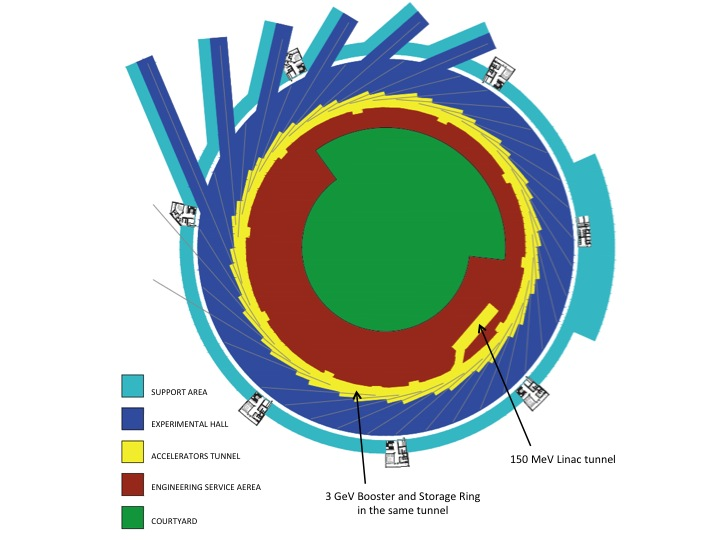
\includegraphics[scale=0.5]{figures/sirius_building.jpg}
    \caption{Sirius building layout~\cite{wiki}.}
    \label{fig:sirius_building}
\end{figure}
\subsection{Magnetic Lattice and Basic Parameters}
The final design for Sirius magnetic lattice is represented in Figure~\ref{fig:sirius_lattice}. It is a 5BA lattice with a natural emittance of \SI{0.25}{\nano\meter\radian} at \SI{3}{\giga\electronvolt} for the bare lattice (without \glspl{id}). With the installation of the planned \glspl{id}, the emittance is expected to be reduced as low as \SI{0.15}{\nano\meter\radian}.
\begin{figure}
    \centering
    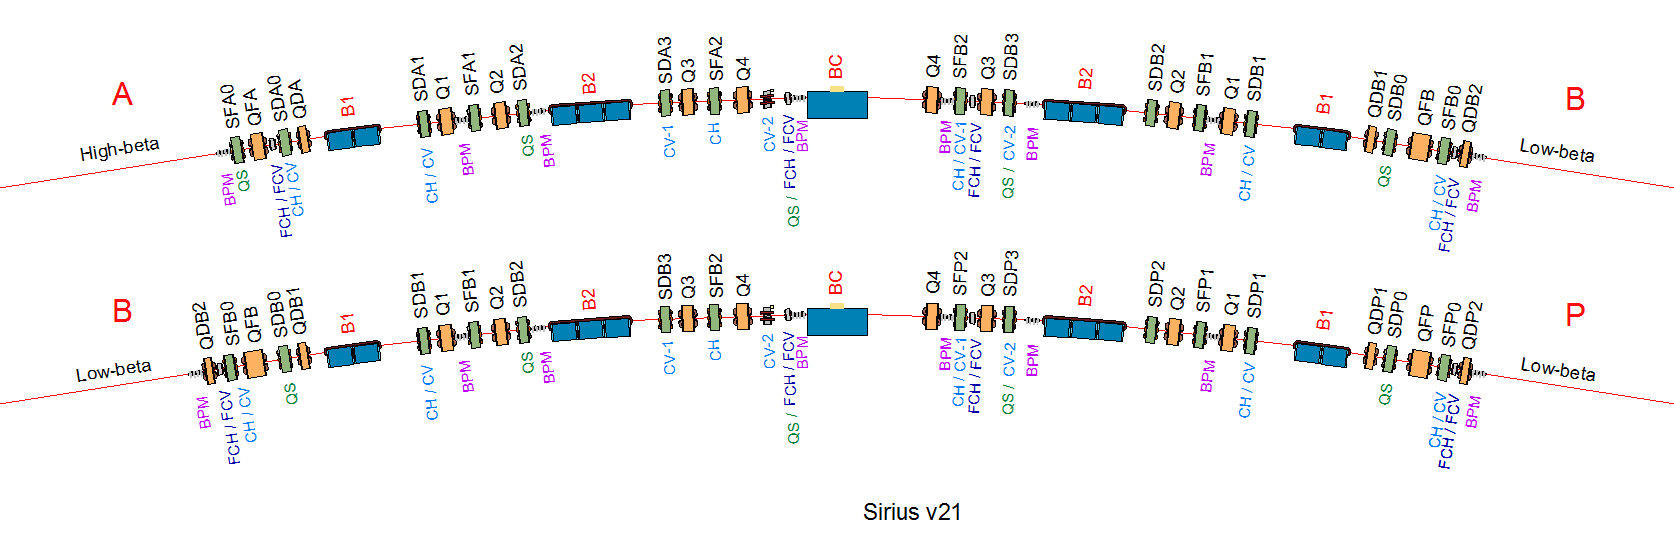
\includegraphics[width=\textwidth, trim={0 2cm 0 0}, clip]{figures/sirius_lattice.png}
    \caption{Sirius 5BA magnetic lattice cells. The magnets are represented by colored blocks. Dipoles (B) are in blue, quadrupoles (Q) in orange and sextupoles (S) in green. The cells are characterized by their straight sections types: high-beta (A) or low-beta (B, P). The Sirius storage ring is composed by 5 super-periods, each one composed by the four cells sequence A-B-P-B~\cite{wiki}.}
    \label{fig:sirius_lattice}
\end{figure}

The optical lattice functions for one superperiod of the Sirius magnetic lattice are plotted in Figure~\ref{fig:twiss_functions}. The small values for the dispersion and betatron functions, especially at the central bending magnet, are fundamental factors to obtain the low emittance in Sirius storage ring. The zero dispersion and the low beta functions in the straight sections, combined with the low emittance, are essential to obtain small beam sizes at beamlines. The zero dispersion also is required to the possibility of emittance reduction after \glspl{id} installation.
\begin{figure}
    \centering
    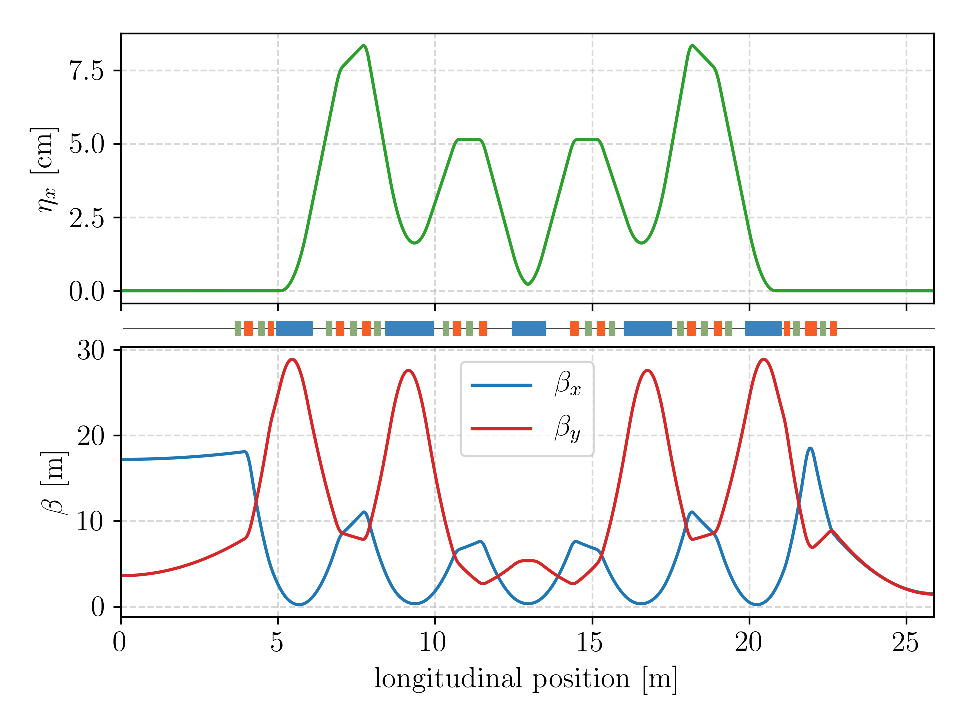
\includegraphics[width=1.0\textwidth]{figures/twiss_plot_refine_lattice_grid.eps}
    \caption{Lattice functions for one 5BA cell for the Sirius storage ring with a high-beta straight section in the left and a low-beta in the right.}
    \label{fig:twiss_functions}
\end{figure}

The Sirius magnetic lattice counts with 20 straight sections, being 5 with high horizontal betatron fuction (A type) and 15 with low horizontal and vertical betatron functions (B and P types). One of the main differentials of Sirius is having that many low-beta straight sections around the storage ring. Regarding the linear lattice elements, the B and P sections are identical and the difference is related to the sextupoles, i.e., second order elements. 17 out of 20 straight sections are available for \glspl{id} installation, 2 will be used for machine installations and 1 will be shared between a small~\gls{id} and machine installation~\cite{liu2019}. 

The central dipole BC is a permanent magnet with a strong peak field of \SI{3.2}{\tesla} and longitudinal gradient. In the storage ring there are 20 of such superbends providing X-rays with critical energy of \SI{19.2}{\kilo\electronvolt}~\cite{Liu2016b} and allowing for additional 20 beamlines. The remaining four dipoles per arc, two B1 and two B2, are electromagnets with peak fields of \SI{0.58}{\tesla}. The total number of dipoles in the Sirius magnetic lattice is $5 \times 20 = 100$, being 20 permanent magnets (BC) and 80 electromagnets (B1 and B2).

The high-beta straight sections count with a quadrupole doublet (QFA, QDA) for the optics matching. In low-beta straight sections quadrupole triplets are used for the matching (QFB, QDB1, QDB2) for B-type section and other triplet (QFP, QDP1, QDP2) for P-type sections. The quadrupoles in the arc sections are labeled as Q1, Q2, Q3 and Q4. Thus, there are 12 families of quadrupoles in the Sirius magnetic lattice. Notice that the quadrupole and dipole magnets in the arc have a mirror symmetry around the BC magnet. The total number of quadrupoles in Sirius storage ring is 270. 

In the Sirius lattice there are 21 families of sextupoles, whose names can be checked in Figure~\ref{fig:sirius_lattice}. Sextupoles are used for the correction of chromatic errors and non-linear dynamics optimization. The number of sextupole magnets in Sirius is 280.

For the slow orbit correction system, there are 8 \glspl{bpm} per arc section, thus totalling $8 \times 20 = 160$ \glspl{bpm} in the storage ring. There are 6 horizontal correctors (CH) and 7 vertical correctors (CV) per section, both types installed in sextupole magnets. There is also 1 additional vertical corrector magnet installed per arc, then there are $6 \times 20 = 120$ CHs and $(7 + 1) \times 20 = 160$ CVs in the storage ring. The orbit correction is presently controlled by the in-house implemented system called~\gls{sofb}.

For the fast orbit correction system, there are 4 horizontal and 4 vertical fast correctors (FCH and FCV, respectively) per sector, so 80 FCH and 80 FCV in total (there are 2 FCH and 2 FCV per source point). The fast orbit correction will be controlled by the Fast Orbit Feedback (FOFB) system.

The coupling control system counts with 4 skew quadrupoles\footnote{A skew quadrupole is basically a normal quadrupole rotated by a $\SI{\pi/4}{\radian}$ angle.} (QS) per arc that are achieve as additional coils in sextupole magnets and 1 additional QS in one fast corrector per section. Hence, there are $(4 + 1) \times 20 = 100$ QS in the storage ring. The 80 skew quadrupoles in sextupole magnets are already sufficient for coupling control and the remaining 20 QS in the fast correctors are used for the process of~\gls{bba}, where the electron beam is used to measure the center offsets between the \glspl{bpm} and the quadrupoles, in order to correct the orbit towards the magnets centers as close as possible. The skew quadrupoles in fast correctors are useful for~\gls{bba} since they are positioned very close to the BPM right next the BC magnet.

Table~\ref{tab:sirius_elements} summarizes the number of elements for each type that are installed in the Sirius storage ring. The main global parameters for the Sirius storage ring can be found in Table~\ref{tab:sirius_main_parameters}, where the relevant parameters for each planned operation phase are presented as well. Much more technical information about Sirius can be accessed in the open website~\cite{wiki}.
\begin{table}
        \centering
        \caption{Number of elements for each type in Sirius storage ring.}
        \label{tab:sirius_elements}
        \begin{tabular}{cc}
            \toprule\toprule
            Element Type & \# of Elements \\
            \hline
            Dipole              & 100 \\
            Quadrupole          & 270 \\
            Sextupole           & 280 \\
            % \hline
            BPM & 160 \\
            H. Slow Corrector & 120 \\
            V. Slow Corrector & 160 \\
            Skew Quadrupole & 100 \\
            % \hline
            H. Fast Corrector & 80 \\
            V. Fast Corrector & 80 \\
            \bottomrule\bottomrule
        \end{tabular}
\end{table}
\begin{table}
        \centering
        \caption{Main parameters of the Sirius storage ring. Adapted from \cite{Sa2018}.}
        \label{tab:sirius_main_parameters}
        \begin{tabular}{lccccl}
            \toprule\toprule
            \mr{2}{*}{Parameter} &  \mr{2}{*}{Symbol} & \mc{3}{c}{Operation Phases}& \mr{2}{*}{Unit}\\\cmidrule{3-5}
                                 &                    &Commiss. & Phase 1 & Phase 2& \\\hline
            Energy               & $E_0$     & \mc{3}{c}{3.0}    & \si{\giga\electronvolt}\\
            Gamma factor         & $\gamma$  & \mc{3}{c}{5871}& \\
            Circumference        & $L_0$     & \mc{3}{c}{518.396}  & \si{\meter}\\
            Revolution period    & $T_0$     & \mc{3}{c}{1.729}   & \si{\micro\second}\\
            Revolution frequency & $f_0$     & \mc{3}{c}{578}    & \si{\kilo\hertz}\\
            Harmonic number      & $h$       & \mc{3}{c}{864}    & \\
            Momentum compaction  & $\alpha$  & \mc{3}{c}{\SI{1.636e-4}{}}& \\
            Transverse tunes (H/V)& $\nu_{x/y}$   & \mc{3}{c}{49.096/14.152}  & \\
            Energy loss per turn & $U_0$     & \mc{3}{c}{471}    & \si{\kilo\electronvolt} \\
            Natural emittance    & $\varepsilon_0$& \mc{3}{c}{251}& \si{\pico\meter\radian} \\
            Natural energy spread& $\sigma_\delta$& \mc{3}{c}{\SI{8.5e-4}}& \\\midrule
            % Damping times (H/V/L)& $\tau_{x/y/z}$ & \mc{3}{c}{16.9/22.0/12.9}& \si{\milli\second}\\
            % Damping rates (H/V/L)& $\alpha_{x/y/z}$ & \mc{3}{c}{59.5/45.8/77.8}& \si{\hertz}\\\midrule
            Nominal total current& $I_0$     & 30    &  100  & 350 & \si{\milli\ampere}\\
            RF cavity            &  & 1 7-Cell & \mc{2}{c}{2 SC-RF}  \\
            Gap voltage          & $\hat{V}_{\mathrm{rf}}$     & 1.8   & \mc{2}{c}{3.0}& \si{\mega\volt} \\
            Natural bunch length & $\sigma_z$& 3.2 (10.7) & \mc{2}{c}{2.5 (8.2)}& \si{\milli\meter} (\si{\pico\second}) \\
            Synchrotron tune     & $\nu_z$& \SI{3.56e-3} & \mc{2}{c}{\SI{4.6e-3}}& \\\bottomrule\bottomrule
        \end{tabular}
    \end{table}

\subsection{Commissioning}
Between the assembly of the synchrotron light source components and the regular operation of the facility there is a gap where a lot of parameters tuning and measurements are made. The final goal is providing the conditions to reliably execute the electron beam journey (from the electron gun at~\gls{linac} until the storage ring) and then to push the machine performance and the electron beam properties to meet the design specifications, reaching the ideal operation conditions. This gap is the commissioning\footnote{Actually, the stages of a synchrotron light source history usually have some overlaps and are not as linear as expected.}. The commissioning also can be divided in stages: commissioning of the sub-systems, machine and beamlines.

The realization of~\glspl{4gsr} imposes challenges in its commissioning as well. For the reasons discussed in Subsection~\ref{subsec:fourth_generation}, a MBA lattice rigorously limits the conditions to store an electron beam. Therefore, studying the commissioning steps beforehand with simulations has become a standard practice at the design stage of~\glspl{4gsr}~\cite{sajaev2015, liuzzo2017, ghasem2019, sajaev2019, hellert2019}, so the challenges and its solutions can be foreseen. 

The author contributed to the Sirius commissioning simulations studies, where simulations for the commissioning procedures with realistic errors were developed and applied both for Sirius booster and storage ring lattice models~\cite{alves2019}. The studies results served as guidelines and procedures that were successfully applied on Sirius commissioning to accumulate a \SI{10}{\milli\ampere} electron beam at \SI{3}{\giga\electronvolt} in the Sirius storage ring for the very first time in February 20, 2020. The author had the singular opportunity to participate in the commissioning stages that led to this achievement.

The commissioning phase in which coarse adjustments are made allowing the electron beam to reach its final condition in the storage ring for the first time is often called early commissioning. At this stage, typically the machine performance optimization is not a major concern, since the feasibility of each process is being proven in first place. Therefore, it can be stated that the Sirius early commissioning has ended in February 20, 2020, proving that were no severe conceptual design errors or problems in the machine assembly that made impossible the electron beam accumulation in the storage ring. However, the commissioning after that is not finished yet, since the errors that move away the actual machine performance and beam properties from the expected and designed values are still present and uncorrected at this stage.

In order to optimize the machine performance, a second stage of the commissioning is needed. At this phase, the electron beam is available for measurements. These machine studies have been carried out by the Sirius commissioning team during the 2020 year. At the time of writing the machine commissioning is currently in progress alongside with the commissioning of 6 beamlines, 5 of them using non-definitive \glspl{apu} as the synchrotron radiation source, which were specifically installed in these beamlines for the commissioning stage, and the remaining beamline uses a superbend BC as the light source. Until the end of 2020, the Sirius operation shifts were alternating between machine and beamline commissioning, where for the latter the storage ring was delivering a \SI{40}{\milli\ampere} electron beam in decay-mode for the beamlines.
% LNLS Accelerator Physics Group is working continuously on the issues related to the machine performance improvements. 
\section{Scientific Background}\label{sec:background}
The storage ring linear optics is fundamental to determine the electron beam equilibrium distribution, then the beam size and divergence depends directly on the linear optics. It also has an effect on the beam stability. Large deviations in the linear optics compared to the nominal optics move away the beam properties from the design values or, more drastically, these errors might preclude to store an electron beam. Typically, most of the optics errors are found in the first commissioning stages of a new storage ring.

Linear optics errors can be caused by various sources. Strength errors in the quadrupole magnets, horizontal orbit offsets in sextupoles, changing the effective focusing on the beam, gradient errors in dipoles, errors in the magnets excitation curves -- the calibration between the current setting in the power supplies and corresponding magnetic fields in the electromagnets. \glspl{id} may introduce gradient errors as well. Deviations in linear optics may break the lattice symmetry, which may introduce additional resonances in the beam dynamics, thus increasing the chances of beam loss.

In a basic description of the transverse dynamics for electrons in a storage ring, the horizontal and vertical motions are uncoupled, thus the transverse planes can be regarded as independent. In this case, the theoretical vertical emittance is almost zero. However, roll errors in the dipoles and quadrupoles, vertical orbit offsets in the sextupoles, random skew gradients errors and \glspl{id} introduce coupling between the transverse planes. The roll errors may also create a vertical dispersion function, which is nominally zero. Therefore, coupling errors increase the vertical beam size and may have an effect on the injection efficiency, by transferring part of the large horizontal amplitude of the injected beam into the vertical plane.  

Even if the errors sources are beforehand minimized as much as possible, with magnets characterization, installation and alignment reaching the specifications, these processes are limited by finite precision and the residual errors may still affect negatively the electron beam. Since the electron beam in a storage ring is a very sensible probe, beam-based techniques are often used for characterization and optimization. Two approaches can be made: (i) perform beam-based measurements related to the linear optics and coupling, and guided by the accelerator physics theory, one can use the storage ring model to calculate the corrections with the design values as the final target; (ii) consider the storage ring as a black-box, then perform parameters variations with the goal to improve a figure of merit constructed with beam-based data. The approach (i) is often called beam-based corrections and the (ii) beam-based optimization~\cite{huang2019beam}.

% The goal for the teams responsible for the storage ring elements fabrication and for its assembly in the tunnel is to deliver a machine for the commissioning team where the residual errors are compatible with the specified tolerances, thus the remaining errors are expected to be corrected with variations in the parameters with intensities also compatible with the correction systems design. After these fine adjustments made during the commissioning, it is expected that the real storage ring performance and properties move towards the design values.

% Measuring the magnetic field errors in the elements after installed in the storage ring, besides being an unrealistic process, it does not provide very useful information, since the corresponding effects in the electron beam and how the beam experiences the fields is what really matters. 
Each approach has its pros and cons but their final goal is the same: improve the machine performance. The beam-based correction approach has the conceptual advantage that, based on the theory, it tries to increase the real accelerator performance by making it as close as possible to the design accelerator. On the other hand, since this method is model-dependent, i.e., it depends on the correspondence between the storage ring modeling and the real storage ring, if the model fails to accurately describe the reality, the corrections effectiveness is reduced or even worse, the intended corrections are manifested as additional perturbations. The beam-based optimizations have the advantage of being model-independent, however depending on the case, the optimization process might take too much time to converge and it also might be more susceptible to noise and variations in the measured data. Moreover, the final corrections obtained by the optimization must be interpreted and explained afterwards, which may not be a trivial task in general.

Linear Orbit from Closed Orbits (LOCO) is a beam-based correction method implemented by J. Safranek and first applied to the National Synchrotron Light Source (NSLS) storage ring~\cite{safranek1994, safranek1995, safranek1997}. The ideas behind LOCO method were developed in previous works at Stanford Linear Accelerator Center (SLAC)~\cite{martin1992, corbett1993}. The main idea of this method is to use the beam orbit response due to localized dipolar fields variations to extract information about the linear optics and coupling in the real machine. This is done by measuring the orbit response with the stored electron beam and then calibrating the model machine to the data, i.e., changing the relevant parameters in the model until the simulated orbit response matches the measured one. After this process, if the model describes reasonably the real storage ring, the actual linear optics and coupling can be derived and its deviations from the nominal values are obtained as well. Furthermore, from the calibrated model it is also possible to calculate the variations for adjustable parameters in the real machine, which allows for the correction of linear optics and coupling errors. In this way, LOCO method can be used both as a diagnostic and a correction tool.

The LOCO code was first implemented in FORTRAN language~\cite{icfa_safranek} and this version was used to correct the optics in the NSLS X-ray ring~\cite{safranek1997} and debug problems in the Advance Light Source (ALS) optics~\cite{robin1996}. Several years later, LOCO code was implemented in MATLAB~\cite{safranek2002, icfa_greg} with a graphical user interface and compatible with the Accelerator Toolbox (AT), an accelerator modelling tool in MATLAB~\cite{terebilo2001}. 

After that, LOCO has become a tool widely applied in many accelerators around the world. UVX, the first synchrotron light source of~\gls{lnls}, was amongst these facilities~\cite{resende2010}. Other improvements in the method were made, adding options of alternative minimization methods and constraints to the fitting~\cite{icfa_huang}. The author in~\cite{icfa_safranek} mentions that, in 2007, after a search for ``LOCO'' in the text of papers on the Joint Accelerator Conferences website~\cite{jacow}, 107 papers were found. The same search made in 2020 yielded 510 results. This illustrates the impact of LOCO method in the accelerator community over the years. LOCO has already been proven to be a useful tool for 4\ts{th} generation light sources as well, after being applied in MAX-IV first optics studies~\cite{leemann2017}.

The effects of LOCO corrections on the machine can be checked by independent beam-based measurements. It can be verified if the measured orbit response converged to the expected orbit response from the nominal lattice. Changing a quadrupole strength and measuring the corresponding shifts in the betatron tunes is a procedure to determine the beta functions at quadrupoles. The beta function at the \glspl{bpm} can be determined by applying a fast dipolar impulse to the beam (for example with a pinger) and measuring the~\gls{tbt} response in the beam trajectory over time. The dispersion function at \glspl{bpm} is determined by varying the~\gls{rf} frequency in the cavity and measuring the variation in the beam orbit. Approximating the horizontal and vertical tunes and measuring its minimum distance allows to determine the global betatron coupling. The magnitude of the measured orbit response in one direction due to a dipolar variation in the perpendicular plane provides the information about the coupling distribution along the storage ring. The strength of the fast dipolar impulse can be increased until the electron beam is partially or completely lost, providing information about the dynamic aperture region. If a diagnostic beamline is available, beam emittance measurements can be performed. The injection efficiency in the storage ring is also a good indicative of performance improvement.
\section{Master's Objectives}\label{sec:master_obj}
The predominant programming language used in Sirius machine control system is Python. After the design studies that resulted in the Sirius lattice and the commissioning simulations, the Sirius models in MATLAB were not satisfactory explored by the~\gls{lnls}~\gls{fac} in the actual commissioning, mainly due to inconveniences related to the different programming languages. Since there were accelerator modeling and simulations Python frameworks developed in-house and in advanced stages of implementation, the full migration of the Sirius to Python regarding the Accelerator Physics modeling and simulations were performed quite rapidly with only small adjustments.
 
Next to this, even though LOCO code is available in MATLAB, the~\gls{lnls}~\gls{fac} was also seeking for an expertise development related to the method proposed in LOCO for the application on Sirius commissioning and later on the machine studies shifts. Moreover, a code developed in-house is much more flexible to test new ideas and to implement new functionalities. Considering the programming language migration as well, the idea of studying LOCO method and implementing the code in Python came naturally. The author had the opportunity to conduct this task, which derived in this master's work. 

The master's main goals can be organized as follows:
\begin{itemize}
    \item Study the Linear Optics From Closed Orbits (LOCO) method.
    \item Implement LOCO in Python for the Sirius storage ring model.
    \item Test the reliability of the implemented code with simulation studies.
    \item Implement a measurement script for the betatron function by tune shifts.
    \item Realize linear optics and coupling studies in the Sirius storage ring during the commissioning, performing measurements and corrections using the implemented codes.
\end{itemize}

To summarize, the master's dissertation gathers the author's contributions to the Sirius storage ring commissioning regarding the first studies and results related to the linear optics and coupling measurements\footnote{Some measurement scripts used in the dissertation are results from collective work of the~\gls{fac}, but the reported measurements were performed by the author during the Sirius commissioning.} and corrections. 










